\documentclass[10pt,twocolumn,twoside,letterpaper]{IEEEtran}

\makeatletter
% \def\ps@IEEEtitlepagestyle{
%   \def\@oddfoot{\mycopyrightnotice}
%   \def\@evenfoot{}
% }
% \def\mycopyrightnotice{
%   {\footnotesize
%   \begin{minipage}{\textwidth}
%   \centering
%   978-1-7281-4164-0/19/\$31.00 \copyright2019 IEEE
%   \end{minipage}
%   }
% }

\ifCLASSINFOpdf
   \usepackage[pdftex]{graphicx}
\else
   \usepackage[dvips]{graphicx}
\fi

\ifCLASSOPTIONcompsoc
  \usepackage[caption=false,font=normalsize,labelfont=sf,textfont=sf]{subfig}
\else
  \usepackage[caption=false,font=footnotesize]{subfig}
\fi

\usepackage{amsmath}
\usepackage{bm}
\usepackage{amssymb}
\usepackage{algorithm}
\usepackage{algorithmic}
\usepackage{stfloats}
\usepackage{url}

\usepackage{geometry}
\geometry{letterpaper, top=0.7in, bottom=0.7in, left=0.65in, right=0.65in}

\usepackage[acronym]{glossaries}
\newacronym{mu-map}{mu-map}{Attenuation Map}
\newacronym{TOF}{TOF}{Time-of-Flight}
\newacronym{nonTOF}{nonTOF}{Non-Time-of-Flight}
\newacronym{NAC}{NAC}{Non-Attenuation Corrected}
\newacronym{RCM}{RCM}{Respiratory Correspondence Model}
\newacronym{MAPE}{MAPE}{Mean Absolute Percentage Error}
\newacronym{COM}{COM}{Centre-of-Mass}
\newacronym{AP}{AP}{Anterior-Posterior}
\newacronym{SI}{SI}{Superior-Inferior}
\newacronym{PET}{PET}{Positron Emission Tomography}
\newacronym{CT}{CT}{Computed Tomography}
\newacronym{MR}{MR}{Magnetic Resonance}
\newacronym{XCAT}{XCAT}{4D Extended Cardiac-Torso}
\newacronym{OSEM}{OSEM}{Orded SubSet Expectation Maximisation}
\newacronym{LOR}{LOR}{Line-of-Responce}
\newacronym{FDG}{FDG}{Fludeoxyglucose}
\newacronym{STIR}{STIR}{Software for Tomographic Image Reconstruction}
\newacronym{SIRF}{SIRF}{Synergistic Image Reconstruction Framework}
\newacronym{FWHM}{FWHM}{Full Width at Half Maximum}
\newacronym{SSD}{SSD}{Sum of Squared Differences}

\usepackage[style=ieee,maxbibnames=19,minbibnames=1,maxcitenames=1,mincitenames=1,backend=biber,defernumbers=false]{biblatex}
\addbibresource{./bibtex/bib/Biblio.bib}

% \IEEEpubid{\begin{minipage}{\textwidth}\ \\[9pt] \centering
% \medskip
% \\
% 978-1-7281-2260-1/19/\$31.00~\copyright~2019~IEEE
% \end{minipage}}

\begin{document}
\title{Impact of Time-of-Flight on Respiratory Motion Modelling using Non-Attenuation-Corrected PET}

\pagestyle{plain}
\pagenumbering{gobble}

\author{Alexander~C.~Whitehead,~\IEEEmembership{Student~Member,~IEEE,}
        Elise~C.~Emond,~\IEEEmembership{Student~Member,~IEEE,}
        Nikos~Efthimiou,~\IEEEmembership{Member~IEEE},
        Adeyemi~Akintonde,
        Scott~W.~Wollenweber,~\IEEEmembership{Senior~Member~IEEE,}
        Charles~W.~Stearns,~\IEEEmembership{Fellow,~IEEE,}
        Brian~F.~Hutton,~\IEEEmembership{Senior~Member,~IEEE,}
        Jamie~R.~McClelland
        and~Kris~Thielemans,~\IEEEmembership{Senior~Member,~IEEE}%

    \thanks{Manuscript recieved 2nd of January 2020.}%
    \thanks{Alexander~C.~Whitehead, Adeyemi~Akintonde and Jamie~McClelland are with the Centre for Medical Image Computing, University College London, London, NW1~2BU, UK.}%
    \thanks{Nikos Efthimiou is with the PET Research Centre, Faculty of Health Sciences, University of Hull, Hull, HU6~7RX, UK.}%
    \thanks{Scott Wollenweber and Charles Stearns are with Molecular Imaging \& Computed Tomography Engineering, GE Healthcare, USA}%
    \thanks{Elise~C.~Emond is supported by GlaxoSmithKline (BIDS3000030921).}%
    \thanks{Jamie R. McClelland is supported by a Cancer Research UK Centres Network Accelerator Award Grant (A21993) to the ART-NET consortium and a CRUK Multi-disciplinary grant (CRC 521).}%
    \thanks{This research is supported by GE Healthcare, the NIHR UCLH Biomedical Research Centre and the EPSRC-funded UCL Centre for Doctoral Training in Medical Imaging (EP/L016478/1).%
    The software used was partly produced by the Computational Collaborative Project in Synergistic PET-MR Reconstruction, CCP PET-MR, UK EPSRC grant EP/M022587/1.}%
    \thanks{This work made use of computational support by CoSeC, the Computational Science Centre for Research Communities.}%
}

\maketitle
\IEEEpeerreviewmaketitle

\begin{abstract}
    Respiratory motion reduces image quality in \gls{PET}. Unless gated \gls{CT} or \gls{MR} data are available, motion correction relies on registration of the \gls{PET} data. To avoid mis-registration due to attenuation mismatches, most existing methods rely on pair-wise registration of \gls{NAC} \gls{PET} volumes. This is a challenging problem due to the low contrast and high noise of these volumes. This paper investigates the possibility of using motion models for respiratory motion correction in \gls{PET}, and in particular whether incorporating \gls{TOF} information increases the accuracy of the motion models derived from the \gls{NAC} reconstructed images. \gls{XCAT} phantom simulations are used for one bed position with a field of view including the base of the lungs and the diaphragm. A \gls{TOF} resolution of 375ps is used. \gls{NAC} images are reconstructed using \gls{OSEM} and used as input for motion model estimation. Different motion models are compared using the original \gls{XCAT} input volumes. The results indicate that \gls{TOF} improves the accuracy of the motion model considerably.
\end{abstract}

\section{Introduction}
\IEEEPARstart{R}{espiratory} motion causes artefacts and loss of resolution in the thoracic region in \gls{PET}~\cite{Nehmeh2008}. Many methods have been proposed to correct for respiratory motion, usually involving registration between a reference volume and a set of volumes in different positions in the respiratory cycle obtained by gating~\cite{Oliveira2014}. However, such pair-wise registration is sensitive to noise. It also does not allow prediction of the respiratory state for data not used to estimate the motion, for instance, to be used for real time motion correction. Surrogate driven motion models attempt to overcome these deficiencies by relating the motion in the data to a number of surrogate signals~\cite{McClelland2013}. The model outputs a transformation or deformation field for every value of the surrogate signals. Motion models are calculated on a series of either time or gating based volumes.

The benefits of using attenuation correction for \gls{PET} image registration are unclear. If images are reconstructed using a static \gls{mu-map}, then artefacts caused by the misalignment between the activity distribution and the \gls{mu-map} would hamper image registration. It could therefore be advantageous to estimate motion on \gls{NAC} images~\cite{WenjiaBai2011}. However, contrast may be too low to calculate an accurate motion model and artefacts associated with the mismatch between the acquisition and system model could also obscure the underlying motion. 

In the absence of \gls{TOF}, there is no information on the activity position along the \gls{LOR} and \gls{NAC} reconstructions have high intensity near the surface and low contrast in the internal part of the body. In \gls{TOF}, the time information constrains the activity position along the \gls{LOR} changing the nature and extent of the artefacts associated with \gls{NAC} as well as changing noise properties~\cite{Ter-Pogossian1981}.

The aim of this work is to investigate whether \gls{TOF} can sufficiently increase the contrast and lower the noise of \gls{NAC} images to facilitate the calculation of accurate motion models.

\section{Methods}
\subsection{XCAT image generation}
\gls{XCAT}~\cite{Segars2010} was used to generate $6$ volumes over a linear $5$ second breathing cycle, with $1$ volume at full expiration at the beginning of the cycle and $1$ volume at full expiration at the end of the cycle and using settings for the extent of Anterior-Posterior (AP) and Superior-Inferior (SI) motion. Activity concentrations were derived from a static \gls{FDG} patient scan. The field of view included the base of the lungs, diaphragm and the top of the liver with a $40$mm diameter spherical lesion placed in the right lung.

\subsection{PET data simulation}
\gls{PET} acquisitions were simulated using \gls{STIR}~\cite{Thielemans2012,Efthimiou2018} through \gls{SIRF}~\cite{ovtchinnikov2019SIRFSynergisticImage,ovtchinnikov_evgueni_2019_3548719} to forward project the input data to sinograms using the geometry of a GE Discovery 710 and, where relevant, a \gls{TOF} resolution of $375$ps similar to the GE Signa PET/MR (using \gls{TOF} mashing to reduce computation time resulting in $13$ \gls{TOF} time bins of size $376.5$ps). Attenuation was included in the simulation using the relevant \gls{mu-map} generated by \gls{XCAT}. Scatter and randoms were not taken into account in the simulation. Multiple noise realisations were generated to simulate an acquisition as if it had been gated into $6$ bins over an acquisition of $120$s, emulating a standard single bed position acquisition. 

\subsection{Image reconstruction}
Data were reconstructed without attenuation correction using \gls{OSEM} with $2$ full iterations and $24$ subsets~\cite{Hudson1994}. Volumes were post filtered using a Gaussian blurring with a kernel size of $6.4$mm \gls{FWHM}.

\subsection{Motion model estimation}
3D B-splines were used to model spatial deformations with the corresponding warping operation denoted as $\mathbf{W}(\mathbf{\alpha}_t)$, with $\mathbf{\alpha}_t$ a vector with B-spline coefficients at time $t$. The breathing surrogate signals $\mathbf{s}$ contained $2$ components, the \gls{AP} and \gls{SI} motion signals used by \gls{XCAT}.  Following~\cite{McClelland2017} a direct correspondence motion model was used where the B-spline coefficients at time $t$ are expressed as a linear combination of the $2$ surrogate signals, $s_{1,t}$ and $s_{2,t}$:

\begin{equation}
    \forall t \in [[1,n_t]],\quad \alpha_{k,t} := R_{1,k} s_{1,t} + R_{2,k} s_{2,t} + R_{3,k}
\end{equation}

\noindent where $\alpha_{k,t}$ is the 3D B-spline coefficient for node $k$ at time point $t$, and $R_{i,k}$ are the model parameters.

A generalised framework unifying image registration and respiratory motion models, NiftyRegResp, was used to estimate the \gls{RCM}s %, which are the object that take in a surrogate signal value and a volume and warp the volume based on the value of the surrogate signal object, of the motion model, 
using \gls{SSD} as an objective function~\cite{McClelland2017}.

\subsection{Evaluation}
We compared $3$ \gls{RCM}s, calculated from the \gls{PET} \gls{XCAT} volumes (gold standard), \gls{nonTOF} \gls{NAC} reconstructions and \gls{TOF} \gls{NAC} reconstructions. To test the accuracy of the \gls{RCM}s, the $3$ models were used to warp the \gls{PET} volume generated by \gls{XCAT} at the mean breathing position to the position at each gate. These estimated volumes were then compared to the original \gls{XCAT} input volumes. Difference volumes were obtained by subtracting the original \gls{XCAT} volume $\mathbf{f}_t$ and warped volumes $\mathbf{W}(\alpha_t) \mathbf{f}_\mathrm{ref}$ at the same gate. \gls{MAPE} were computed from these difference images.

In addition, the \gls{COM} of the lesion was also tracked over the $6$ gates, by warping a volume only including the lesion in the reference position as above, and then computing the \gls{COM}.

\section{Results}
\begin{figure*}
    \centering
    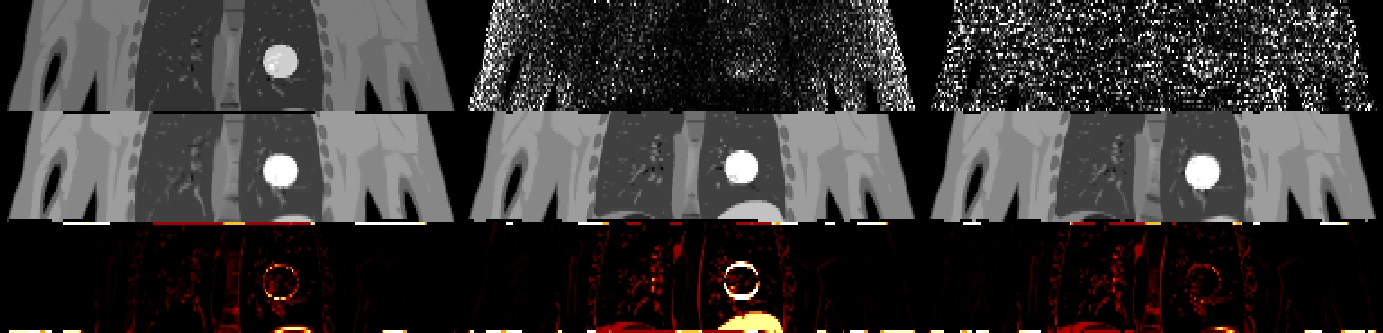
\includegraphics[width=1.0\linewidth]{figures/output.png}
    \captionsetup{singlelinecheck=false, justification=centering}
    \caption{All volumes correspond to end-inhalation. First row from left to right: \gls{XCAT} \gls{PET} data, \gls{NAC} \gls{nonTOF} reconstructed data and \gls{NAC} \gls{TOF} reconstructed data. Second row: \gls{RCM} applied to mean position \gls{XCAT} data with \gls{RCM} derived from \gls{XCAT} \gls{PET} data (left), \gls{NAC} \gls{nonTOF} (middle) and \gls{NAC} \gls{TOF} (right) volumes. Colour map ranges are consistent for all images on this row. The third row from left to right: The difference between the estimated volumes from the second row with the \gls{XCAT} end-inhalation volume. Colour map ranges are consistent for all images on this row.}
    \label{fig:output}
\end{figure*}

\begin{table}
    \centering
    \captionsetup{singlelinecheck=false, justification=centering}
    \caption{Comparison of the \gls{MAPE} between the ground truth data and the volumes estimated from the \gls{XCAT} based \gls{RCM}, the volumes estimated from the \gls{NAC} \gls{nonTOF} based \gls{RCM} and the volumes estimated from the \gls{NAC} \gls{TOF} based \gls{RCM}.}
    
    \resizebox*{1.0\linewidth}{!}
    {
        \begin{tabular}{||c|ccc||}
        \hline
        \textbf{\gls{MAPE}} & \textbf{XCAT} & \textbf{\gls{nonTOF}} & \textbf{\gls{TOF}} \\
        \hline
        \textbf{$1$} & $1.95$ & $8.35$ & $4.18$ \\
        \textbf{$2$} & $1.59$ & $1.61$ & $1.84$ \\
        \textbf{$3$} & $2.06$ & $9.91$ & $5.23$ \\
        \textbf{$4$} & $1.97$ & $6.15$ & $3.68$ \\
        \textbf{$5$} & $1.65$ & $4.45$ & $2.52$ \\
        \textbf{$6$} & $1.95$ & $8.35$ & $4.18$ \\
        \hline
        \textbf{Mean} & $1.86$ & $6.47$ & $3.60$ \\
        \hline
    \end{tabular}
    }
    \label{tab:mape}
\end{table}

\begin{figure}
    \centering
    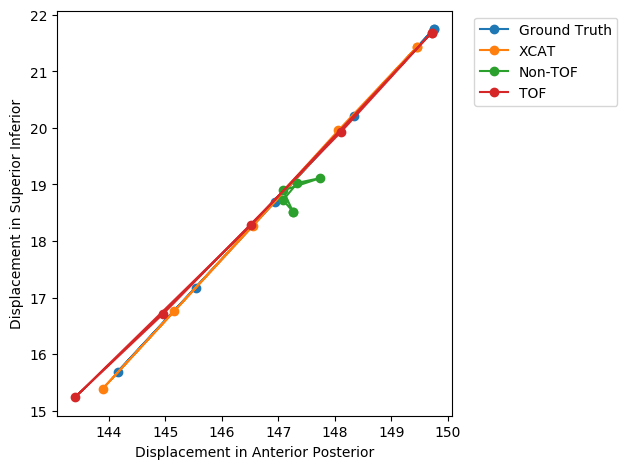
\includegraphics[width=1.0\linewidth]{figures/TOF.png}
    \captionsetup{singlelinecheck=false, justification=centering}
    \caption{The path of the \gls{COM} of the lesion. Horizontal (respectively vertical) axis corresponds to motion in the \gls{AP} (respectively \gls{SI}) direction over the $6$ gates. Different curves denote \gls{COM} displacement for  ground truth data, the estimated data from the \gls{XCAT} based \gls{RCM}, the estimated data from the \gls{NAC} \gls{nonTOF} based \gls{RCM} and the estimated data from the \gls{NAC} \gls{TOF} based \gls{RCM}.}
    \label{fig:com_graph}
\end{figure}

 The reconstructed data, estimated volumes and difference can be seen in Fig~\ref{fig:output} and \gls{MAPE} are in Table~\ref{tab:mape}. The mean \gls{MAPE} was found to be lower for the \gls{NAC} \gls{TOF} data than for the \gls{NAC} \gls{nonTOF}.

 \gls{COM} results can be seen in Fig~\ref{fig:com_graph}. The path of the \gls{NAC} \gls{TOF} data follows the ground truth path much closer than the \gls{NAC} \gls{nonTOF} data, and is quite close to the gold standard \gls{XCAT}-derived motion.

\section{Discussion and Conclusions}
Motion models derived from \gls{NAC} \gls{TOF} volumes were found to be more robust than when using \gls{NAC} \gls{nonTOF}, both visually and when comparing \gls{MAPE} and \gls{COM}. This was noticeable for the lung lesion in the thoracic cavity but also for other parts of the anatomy such as the liver. This is likely due to the improved image contrast of \gls{NAC} \gls{TOF} images.

In the future, research will focus on investigating the robustness of the motion model estimation to different noise levels, acquisition duration and size of lesion.

\AtNextBibliography{\scriptsize}
\printbibliography

\end{document}
